\section{双 Bruhat 胞腔上的可积系统：例子}

\newcommand{\chfHex}[2]{%
  \draw (#1-0.75,#2+0.7)--(#1,#2+0.7)--(#1+0.75,#2)--(#1+0.75,#2-0.7)--(#1,#2-0.7)--(#1-0.75,#2)--cycle;
  \draw (#1,#2+0.7)--(#1,#2+1.2);
  \draw (#1+0.22,#2+0.52)--(#1+0.72,#2+1.0);
  \draw (#1+0.75,#2)--(#1+1.2,#2);
  \node[vb] at (#1-0.75,#2+0.7) {};
  \node[vw] at (#1,#2+0.7) {};
  \node[vb] at (#1+0.75,#2) {};
  \node[vw] at (#1+0.75,#2-0.7) {};
  \node[vb] at (#1,#2-0.7) {};
  \node[vw] at (#1-0.75,#2) {};}

\subsection{三角形}

考虑 Newton 多边形（本例中只是一个三角形），其顶点为 $(-1,0)$、$(0,1)$ 与 $(1,-1)$，面积 $S=3/2$，见图 1.10A。相应的 Thurston 图绘于图 1.10B，其各条线平行于三角形的边。基本域内的三个独立三重点（triple intersection），若三角形的边取逆时针定向，可以分别对应于生成元 $s_0$、$s_1$ 以及再次的 $s_0$，于是相应的 Poisson 子流形由词 $u=s_0s_1s_0\Lambda$ 描述，它是 $\hat A_1$ 的余扩张外尔群的一个元素。

\setcounter{figure}{9}
\begin{figure}[htbp]
\centering
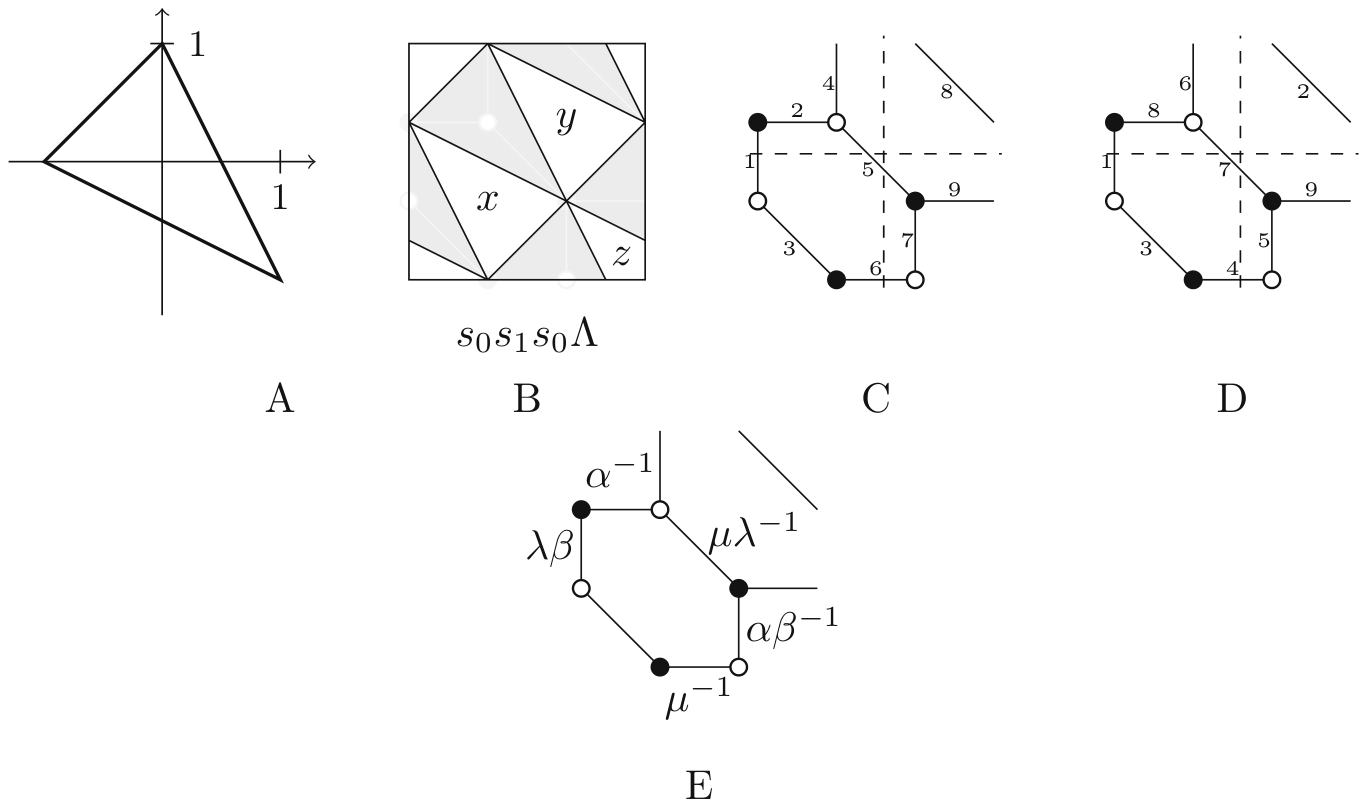
\includegraphics[width=360.9pt]{figs/f1-10.png}
\caption{三角形。A：Newton 多边形 $\Delta$；B：带面变量的 Thurston 图；C：二部图 $\Gamma$；D：对偶环面上的二部图 $\Gamma$；E：边变量与定义二次型的圈。}
\label{fig:1.10}
\end{figure}

相应的三价图 $\Gamma$ 见图 1.10C。本例中对偶曲面 $\tilde\Sigma$ 也是环面，图的嵌入彼此同构。

面变量 $\{x,y,z: xyz=1\}$ 之间的 Poisson 括号由图 1.10B 得出（按附录 1.12 中图 1.23B 构造交换矩阵的规则）：$\{x,y\}=3xy$，$\{y,z\}=3yz$，$\{z,x\}=3yz$。\begin{annote}末式 $\{z,x\}=3yz$ 的比例系数与同列表中前两式（$\{x,y\}=3xy$、$\{y,z\}=3yz$）的循环对称性不合，按循环次序疑应作 $\{z,x\}=3zx$；译文照排原文。[来源：上下文推断]\end{annote}截面 $H^1(\Sigma)\times H^1(\tilde\Sigma)\to C^1(\Gamma)$ 见图 1.10E。这里 $\lambda$、$\mu$ 是 $H^1(\Sigma)$ 上的坐标，$\alpha$、$\beta$ 是 $H^1(\tilde\Sigma)$ 上的坐标，而空间 $C^1$ 在本例中是平凡的。图 1.10C 与图 1.10D 分别画出了 $\Sigma$ 与 $\tilde\Sigma$ 的同调基中的圈，边上的变量只表明这些圈与图的各条边的交点。我们给每个变量配一条虚线圆圈，并把它放在被该圈相交的那些边上。

\begin{figure}[htbp]
\centering
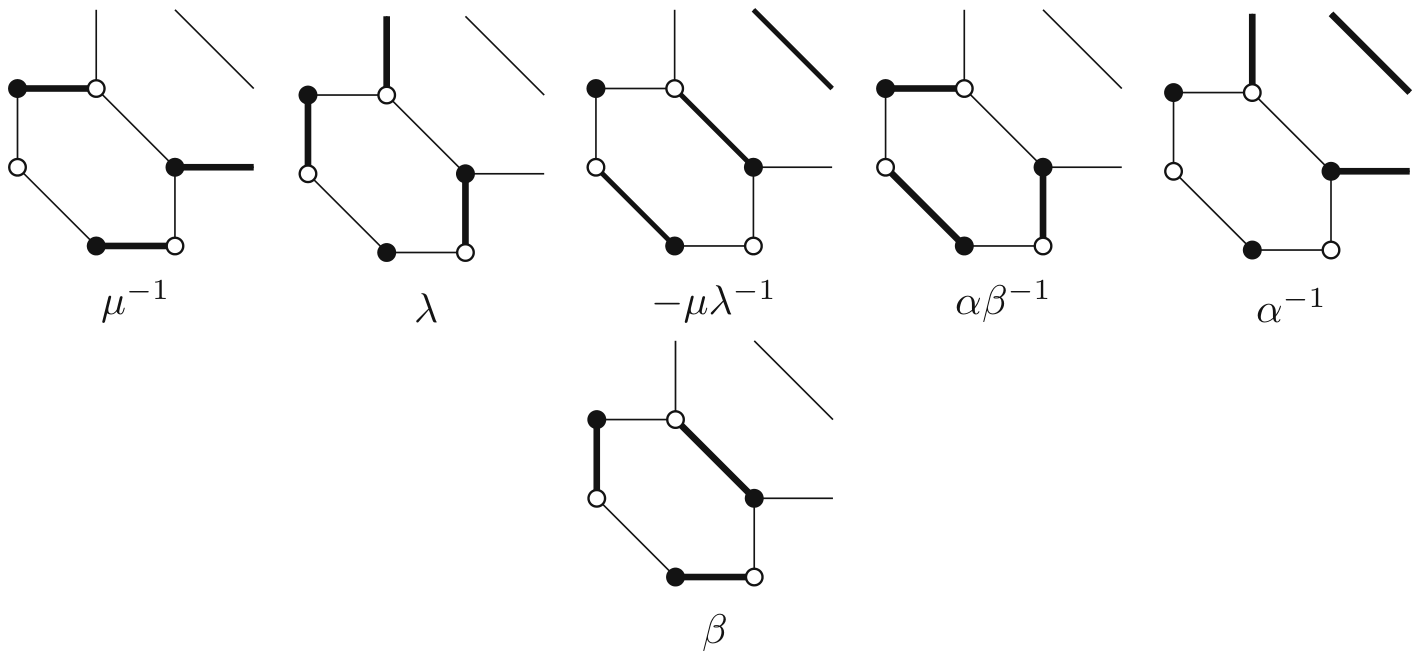
\includegraphics[width=374.9pt]{figs/f1-11.png}
\caption{二聚体构型及相应的配对 $(-1)^{Q(D)}\langle A,D\rangle$。}
\label{fig:1.11}
\end{figure}

该图上有六个二聚体构型，见图 1.11，它们求和得到如下的双配分函数（double partition function）：
\begin{equation}
S^d=\mu^{-1}+\lambda-\mu\lambda^{-1}+\alpha^{-1}+\beta+\alpha\beta^{-1}.
\tag{1.36}\label{eq:1.36}
\end{equation}

同一表达式也可以作为 Dirac 算子（Dirac operator）
\[
\mathfrak D=\begin{pmatrix}
1&1&-\lambda\beta\\
\mu\lambda^{-1}&\alpha^{-1}&1\\
\alpha\beta^{-1}&-\mu^{-1}&1
\end{pmatrix}
\]
的行列式 $S^d=\det\mathfrak D$ 得到，它可以从图 1.10E 读出。（我们选取 Kasteleyn 标号的方式，使得符号被精确复现，而不只是在等价意义下。）

解出联系 $H^1(\tilde\Sigma)$ 与 $B^2(\Sigma)$ 的方程（应当沿图 1.10E 中的各个面取乘积，并计及边的典范定向），得 $x=\alpha\beta^{-2}$，$y=\alpha\beta$，$z=\alpha^{-2}\beta$；把 $\alpha$、$\beta$ 的结果代入表达式 (1.36)，即得归一化面配分函数
\[
S^f=\lambda^{-1}+\mu-\lambda\mu^{-1}+x^{-1/3}y^{-2/3}+x^{-1/3}y^{1/3}+x^{2/3}y^{1/3}.
\]

另一方面，相应矩阵乘积的特征多项式为
\[
\begin{aligned}
A(\lambda,\mu;x,y,z)&=\det(H_0(x)E_0H_1(y)E_1H_0(z)E_0\Lambda-\mu)\\
&=\det\Bigl[\begin{pmatrix}1&0\\ \lambda x&1\end{pmatrix}
\begin{pmatrix}y&0\\0&1\end{pmatrix}
\begin{pmatrix}1&1\\0&1\end{pmatrix}
T_xT_yT_z
\begin{pmatrix}1&0\\ \lambda&1\end{pmatrix}
\begin{pmatrix}0&1\\ \lambda&0\end{pmatrix}
-\mu\Bigr]\\
&=\mu^2-\lambda y-\mu\lambda^2xy-\lambda\mu(1+y+xy).
\end{aligned}
\]

作替换 $\lambda\mapsto\lambda x^{-2/3}y^{-1/3}$、$\mu\mapsto\mu x^{-1/3}y^{1/3}$ 进行归一化，再把结果乘以 $-x^{2/3}y^{-2/3}\lambda^{-1}\mu^{-1}$，就得到同一配分函数表达式。

本例中群 $\mathcal G'_\Delta=\mathcal G_\Delta$ 就是 $\Z/3\Z$，由变量显然的循环置换 $(x,y,z)\mapsto(y,z,x)$ 生成，后者对应于群 $\mathcal G'_\Delta$ 的元素 $(0,1,0)$。

\subsection{最简单的相对论 Toda 链}

下一个例子中 Poisson 结构的秩仍是 2，但与三角形的情形不同，这里存在非平凡的卡西米尔函数（Casimir function）。

\begin{figure}[htbp]
\centering
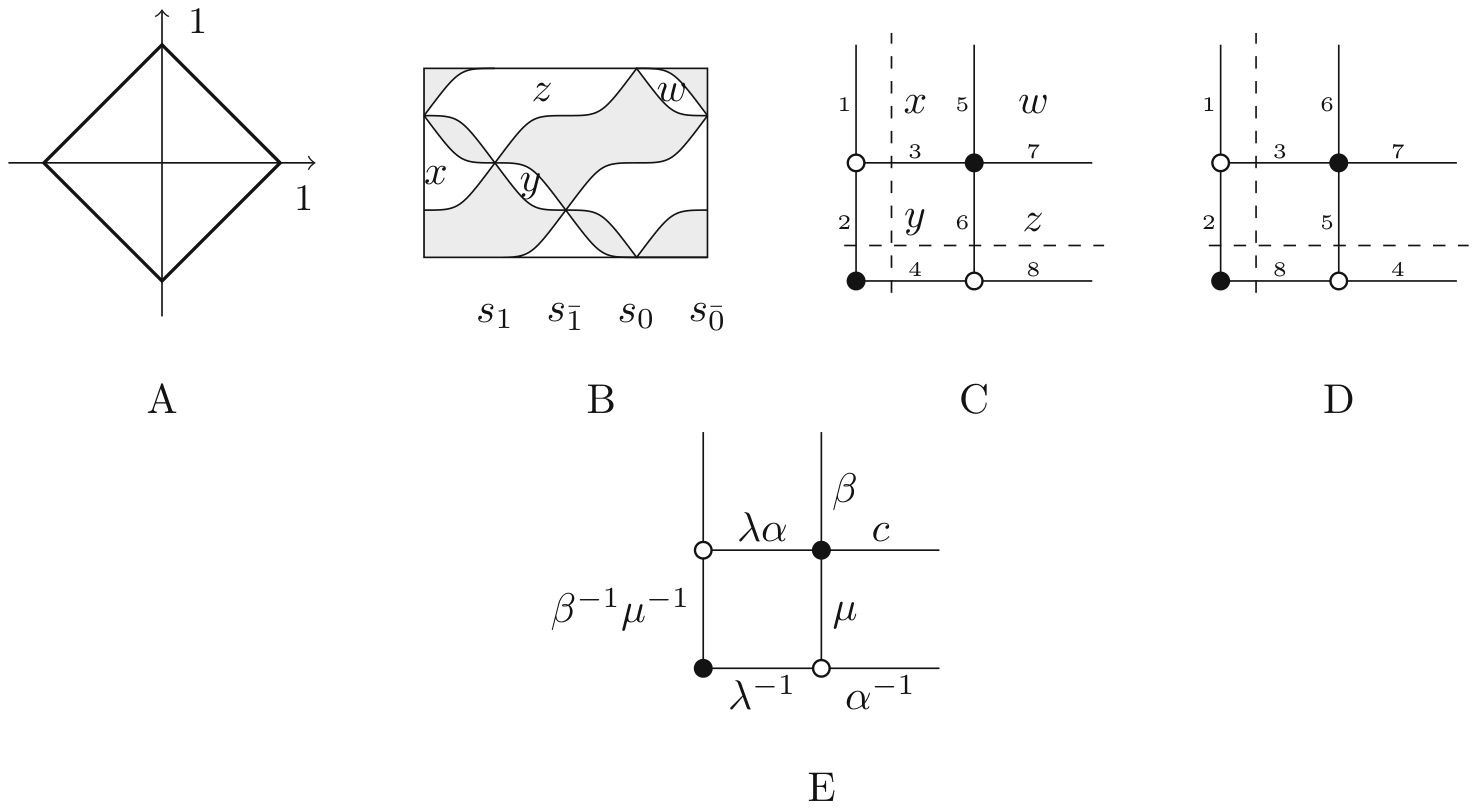
\includegraphics[width=380.0pt]{figs/f1-12.png}
\caption{两粒子相对论 Toda 链。A：Newton 多边形；B：带面变量的 Thurston 图；C：缩并二价顶点后的二部图；D：对偶环面 $\tilde\Sigma$ 上的二部图；E：边变量与定义二次型的圈。}
\label{fig:1.12}
\end{figure}

考虑顶点为 $(1,0)$、$(0,1)$、$(-1,0)$ 与 $(0,-1)$ 的 Newton 多边形，见图 1.12A；其 Thurston 图绘于图 1.12B。

面变量之间的 Poisson 括号由图 1.12B 得出（同样按附录 1.12 中图 1.23B 的通用规则）：$\{x,y\}=2xy$，$\{y,z\}=2yz$，$\{z,w\}=2zw$，$\{w,x\}=2wx$，$\{x,z\}=\{y,w\}=0$。$H^1(\Sigma)=\{(\lambda,\mu)\}$ 到 $H^1(\Gamma)$ 的嵌入例如由 $A_3=\lambda$、$A_4=\lambda^{-1}$、$A_6=\mu$、$A_2=\mu^{-1}$ 以及其余所有 $A_e=1$ 给出（参看图 1.12C 与图 1.12E）。类似地，$H^1(\tilde\Sigma)=\{(\alpha,\beta)\}$ 的嵌入由 $A_3=\alpha$、$A_8=\alpha^{-1}$、$A_5=\beta$、$A_2=\beta$ 以及其余所有 $A_e=1$ 给出，该嵌入可从图 1.12D 读出。\begin{annote}此处 $A_2$ 先被取为 $\mu^{-1}$、又被取为 $\beta$，同一条边不能同时取两个值，底本疑有笔误；译文照排原文。[来源：上下文推断] \end{annote}

卡西米尔空间 $C^1$ 是一维的；我们把卡西米尔函数（Toda 链中的耦合常数）记作 $c$，并把它放在边 7 上，即 $A_7=c$。

\begin{figure}[htbp]
\centering
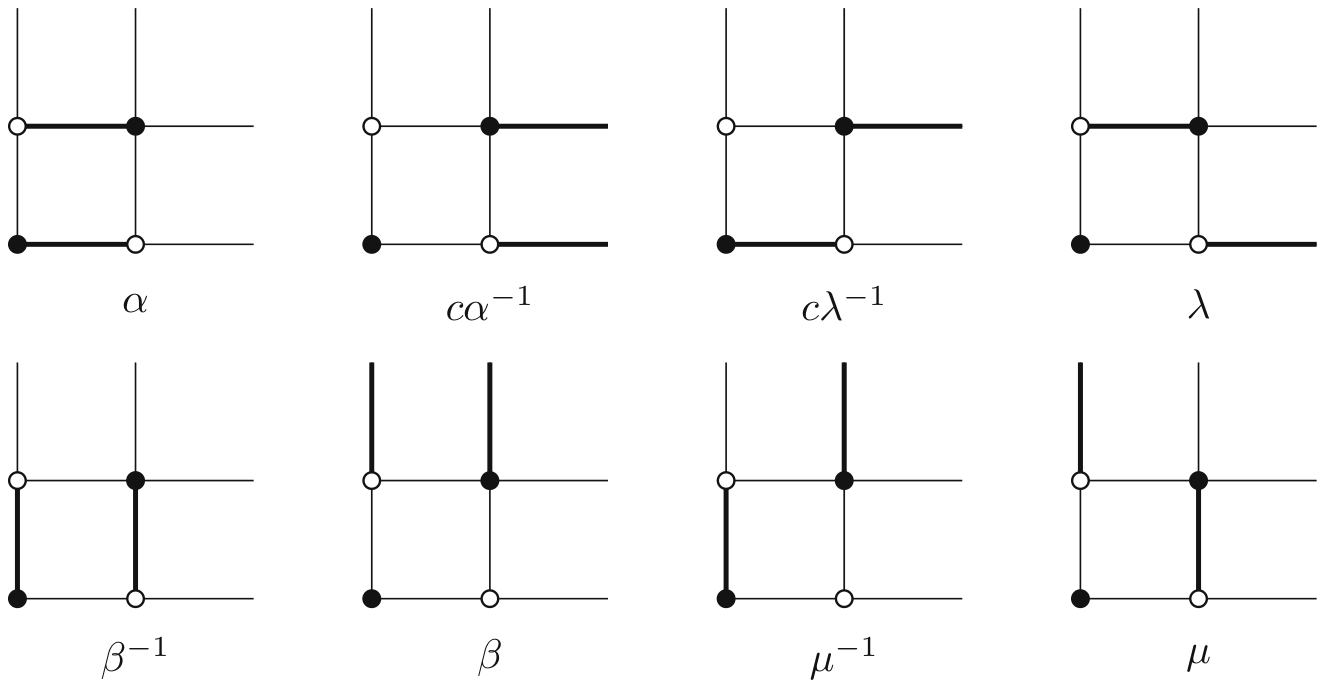
\includegraphics[width=349.8pt]{figs/f1-13.png}
\caption{图 1.12C 中图的二聚体构型。}
\label{fig:1.13}
\end{figure}

该图上有八个二聚体构型，绘于图 1.13，它们给出如下双配分函数\footnote{值得指出的是，仅此式在其量子版本下就会给出 Hofstadter 模型 [13] 的一个非平凡谱问题。我们计划另文回到这一问题。}：
\begin{equation}
S^d=\alpha+c\alpha^{-1}+\beta+\beta^{-1}+\lambda+c\lambda^{-1}+\mu^{-1}+\mu.
\tag{1.37}\label{eq:1.37}
\end{equation}

由图 1.12C 与图 1.12E 得到联系 $H^1(\tilde\Sigma)$ 与 $B^2(\Sigma)$ 的方程，解之得 $x=\alpha\beta^{-1}$，$y=\alpha^{-1}\beta^{-1}$，$z=c\alpha^{-1}\beta$，$w=c^{-1}\alpha\beta$。由于 $c=xz=(yw)^{-1}$，作变量替换 $\alpha=c^{1/2}x^{1/2}w^{1/2}=x^{1/2}y^{-1/2}$，$\beta=z^{1/2}w^{1/2}=x^{-1/2}y^{-1/2}$。把这些变量代入配分函数 (1.37)，即得归一化面配分函数
\begin{equation}
S^f=x^{1/2}y^{-1/2}+cx^{-1/2}y^{1/2}+x^{1/2}y^{1/2}+x^{-1/2}y^{-1/2}+\lambda+c\lambda^{-1}+\mu+\mu^{-1}.
\tag{1.38}\label{eq:1.38}
\end{equation}

另一方面，相应矩阵乘积的特征多项式可以这样计算：
\[
\begin{aligned}
A(\lambda,\mu;x,y,z,w)&=\det\bigl[H_1(x)E_1H_1(y)E_{\bar1}H_0(z)E_0H_0(w)E_{\bar0}-\mu\bigr]\\
&= \det\left[\begin{pmatrix}x&0\\0&1\end{pmatrix}
\begin{pmatrix}1&1\\0&1\end{pmatrix}
\begin{pmatrix}y&0\\0&1\end{pmatrix}
\begin{pmatrix}1&0\\1&1\end{pmatrix}\right.\\
&\qquad\qquad\left.\times T_xT_yT_zT_w
\begin{pmatrix}1&0\\ \lambda/w&1\end{pmatrix}
\begin{pmatrix}1&\lambda^{-1}\\0&1\end{pmatrix}
-\mu\right]\\
&=\det\Bigl[\begin{pmatrix}
xy+x+\lambda w^{-1}x&\lambda^{-1}xy+\lambda^{-1}x+xw^{-1}+x\\
1+\lambda w^{-1}&\lambda^{-1}+w^{-1}+1
\end{pmatrix}-\mu\Bigr]\\
&=\mu^2-\mu(w^{-1}+1+x+xy)-\lambda\mu w^{-1}x-\lambda^{-1}\mu+xy.
\end{aligned}
\]

作替换 $w=c^{-1}y^{-1}$，按 $\lambda\to x^{-1/2}y^{-1/2}c^{-1}\lambda$、$\mu\to-x^{1/2}y^{1/2}\mu$ 归一化，再把该表达式乘以 $(xy\mu)^{-1}$，就恰好复现归一化二聚体面配分函数 (1.38)。

\begin{figure}[htbp]
\centering
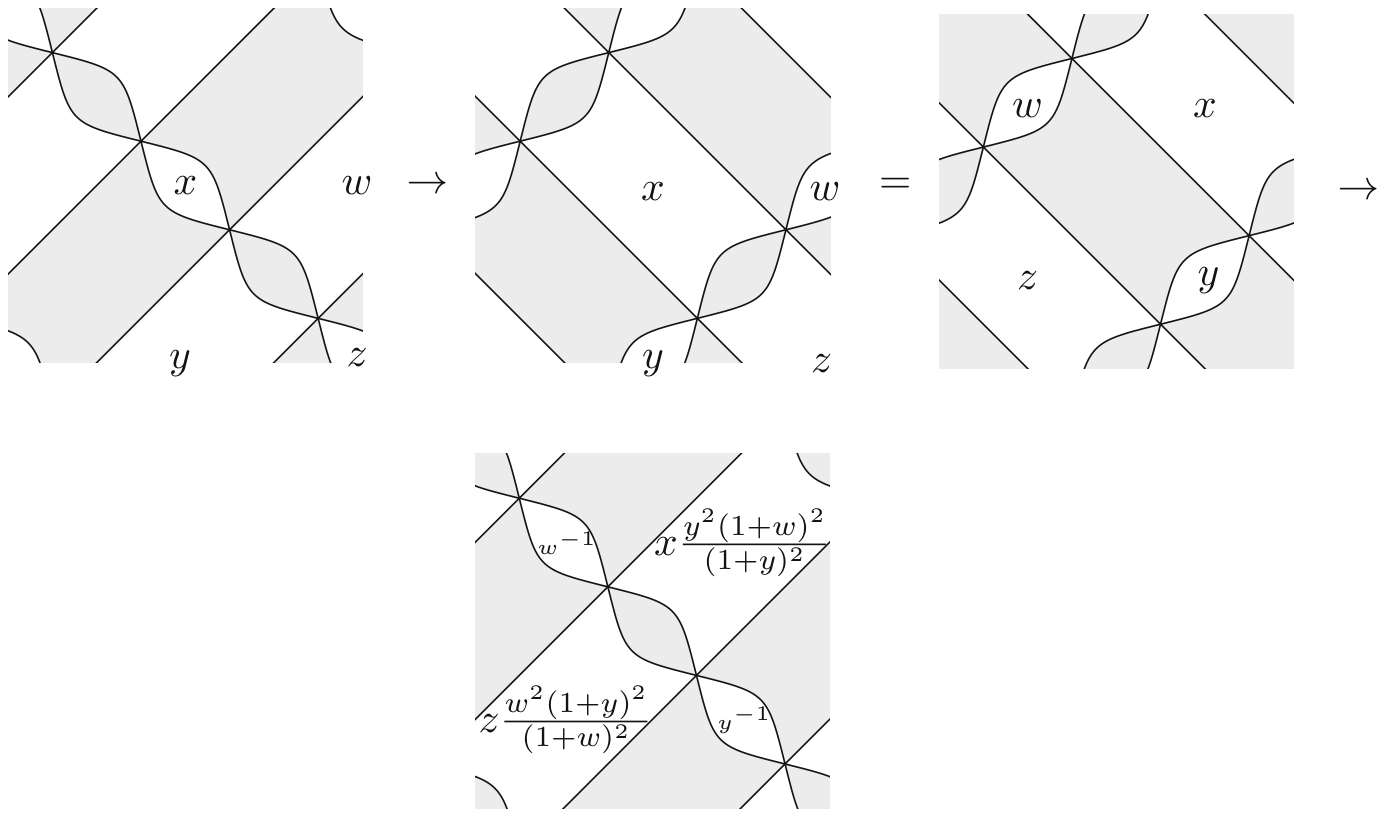
\includegraphics[width=365.6pt]{figs/f1-14.png}
\caption{离散流。第一步是两个灰变异的复合，第二步只是基本域的变换，第三步是两个白变异的复合。}
\label{fig:1.14}
\end{figure}

群 $\mathcal G'_\Delta$ 是秩为 1、挠为 $\Z/2\Z$ 的群。挠生成元 $(1,1,0,0)$ 由坐标置换 $(x,y,z,w)\mapsto(z,w,x,y)$ 给出。无限阶生成元 $(0,1,0,0)$ 由
\[
(x,y,z,w)\mapsto\Bigl(w^{-1},\ zw^2\frac{(1+y)^2}{(1+w)^2},\ y^{-1},\ xy^2\frac{(1+w)^2}{(1+y)^2}\Bigr)
\]
给出，它对应于两次灰变异与两次白变异，如图 1.14 所示。

\subsection{退化到非仿射 Toda 系统}

这个例子说明：对应于较小 Newton 多边形的可积系统，可以由较大的多边形经由某种退化过程得到。考虑这个例子的另一个原因是，它在形式上不属于 GK 方案 [11]，因为相应的二部图在他们的意义下不是极小的。

\begin{figure}[htbp]
\centering
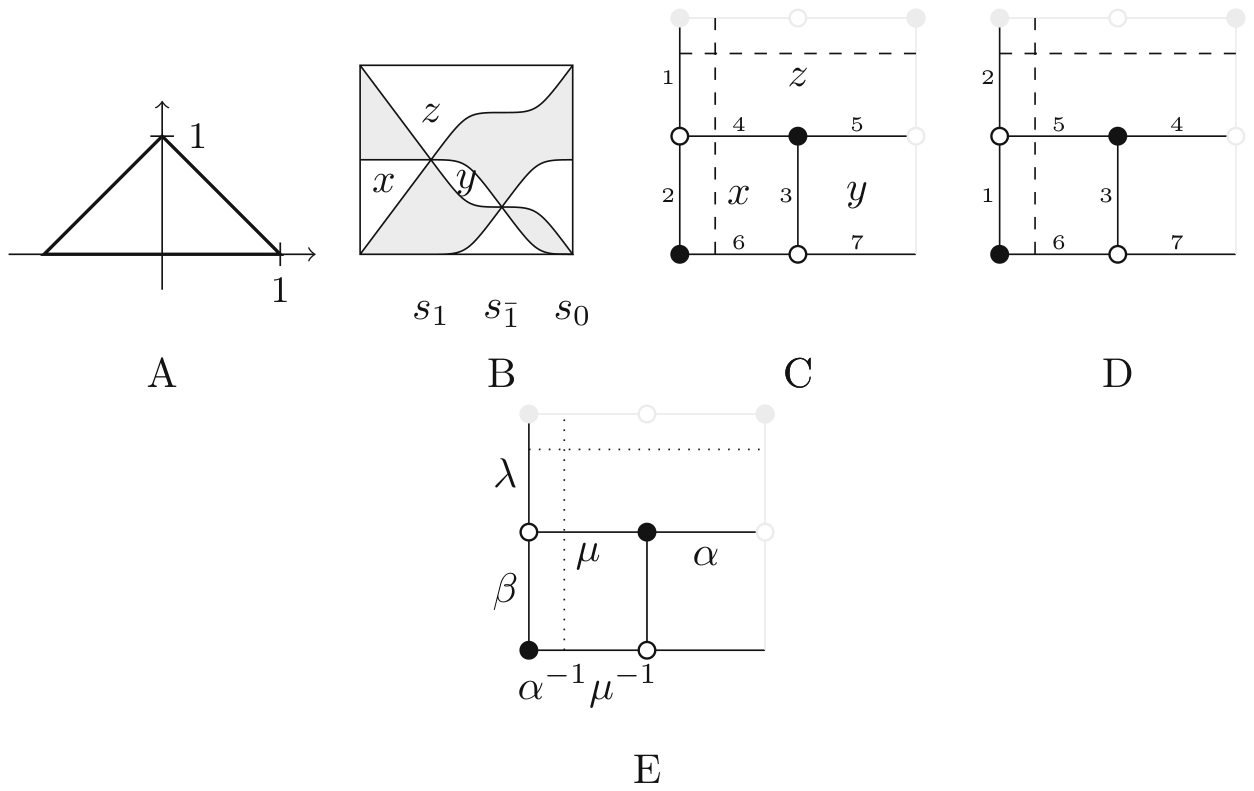
\includegraphics[width=331.1pt]{figs/f1-15.png}
\caption{非仿射的相对论两粒子 Toda 链。A：Newton 多边形；B：Thurston 图；C：环面 $\Sigma$ 上的二部图与同调基；D：对偶环面 $\tilde\Sigma$ 上的二部图与同调基；E：边变量。}
\label{fig:1.15}
\end{figure}

考虑顶点为 $(-1,0)$、$(1,0)$、$(0,1)$、面积 $S=1$ 的 Newton 多边形（三角形），见图 1.15A。图 1.16 中画出了六个二聚体构型，相应的双配分函数为
\[
S^d=\alpha+\alpha^{-1}+\beta+\mu+\mu^{-1}+\lambda.
\]

\begin{figure}[htbp]
\centering
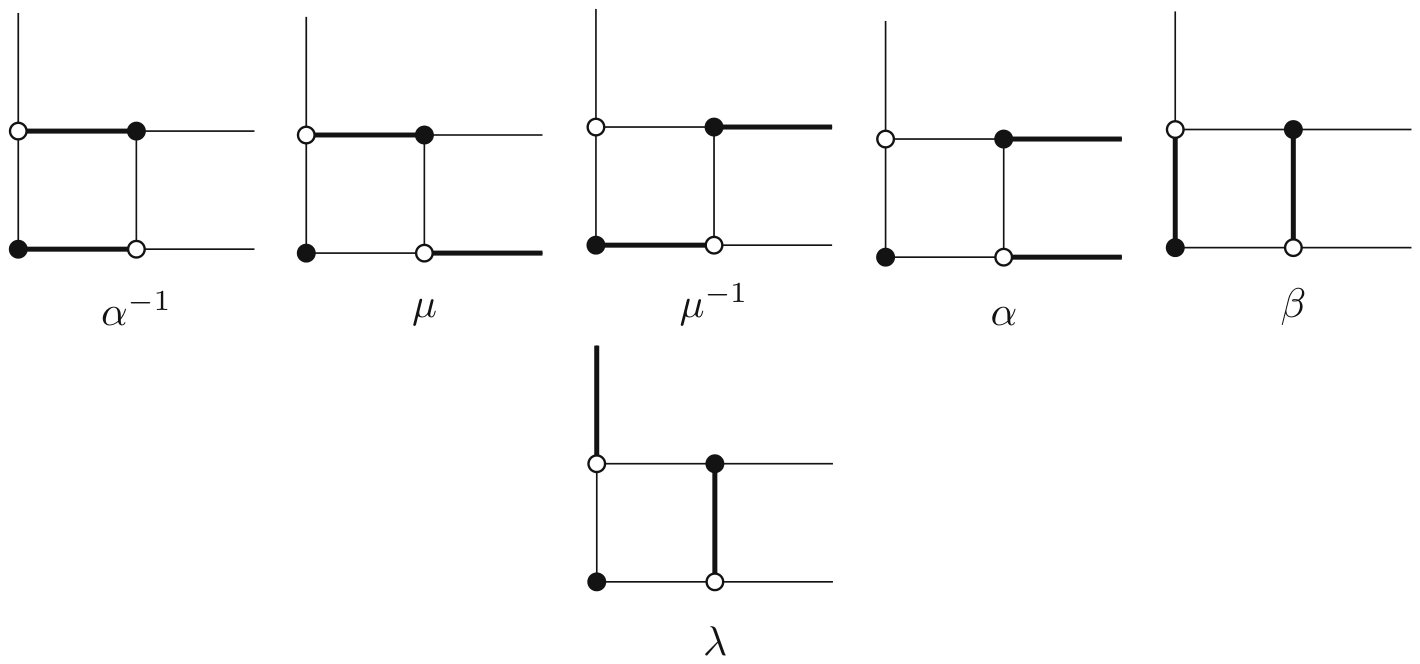
\includegraphics[width=374.9pt]{figs/f1-16.png}
\caption{最简非仿射 Toda 系统的二聚体构型。}
\label{fig:1.16}
\end{figure}

簇变量与面变量之间的关系为 $x=\beta\alpha$，$y=\alpha\beta^{-1}$，$z=\alpha^{-2}$。于是归一化面配分函数为
\begin{equation}
S^f=y^{1/2}x^{1/2}+y^{-1/2}x^{-1/2}+y^{-1/2}x^{1/2}+\mu+\mu^{-1}+\lambda,
\tag{1.39}\label{eq:1.39}
\end{equation}
它应当与特征多项式
\[
\det(H_1(x)E_1H_1(y)E_{\bar1}H_0(z)E_0(\lambda)-\mu)=\mu^2-\mu(1+x+yx)-\lambda\mu x+yx
\]
给出的结果一致。确实，把右端按替换 $\mu\to-y^{1/2}x^{1/2}\mu$、$\lambda\to y^{1/2}x^{-1/2}\lambda$ 归一化，再除以 $\mu yx$，就回到表达式 (1.39)。

可以看出，本例中谱曲线是有理的，它可以按照 [1, 20] 的精神，由最简仿射相对论 Toda 的椭圆曲线 (1.38) 退化得到；事实上，在 (1.38) 中取极限 $c\to0$ 就恰好得到 (1.39)。

\subsection{秩为二的相对论 Toda 链}

前两个例子中 §1.6 的可积系统都是平凡的，因为相空间是二维的，而它只有一个运动积分：哈密顿量。现在我们来考虑具有多于一个交换可积流的最简例子：相空间为四维、有两个独立运动积分的相对论 Toda 链。

\begin{figure}[htbp]
\centering
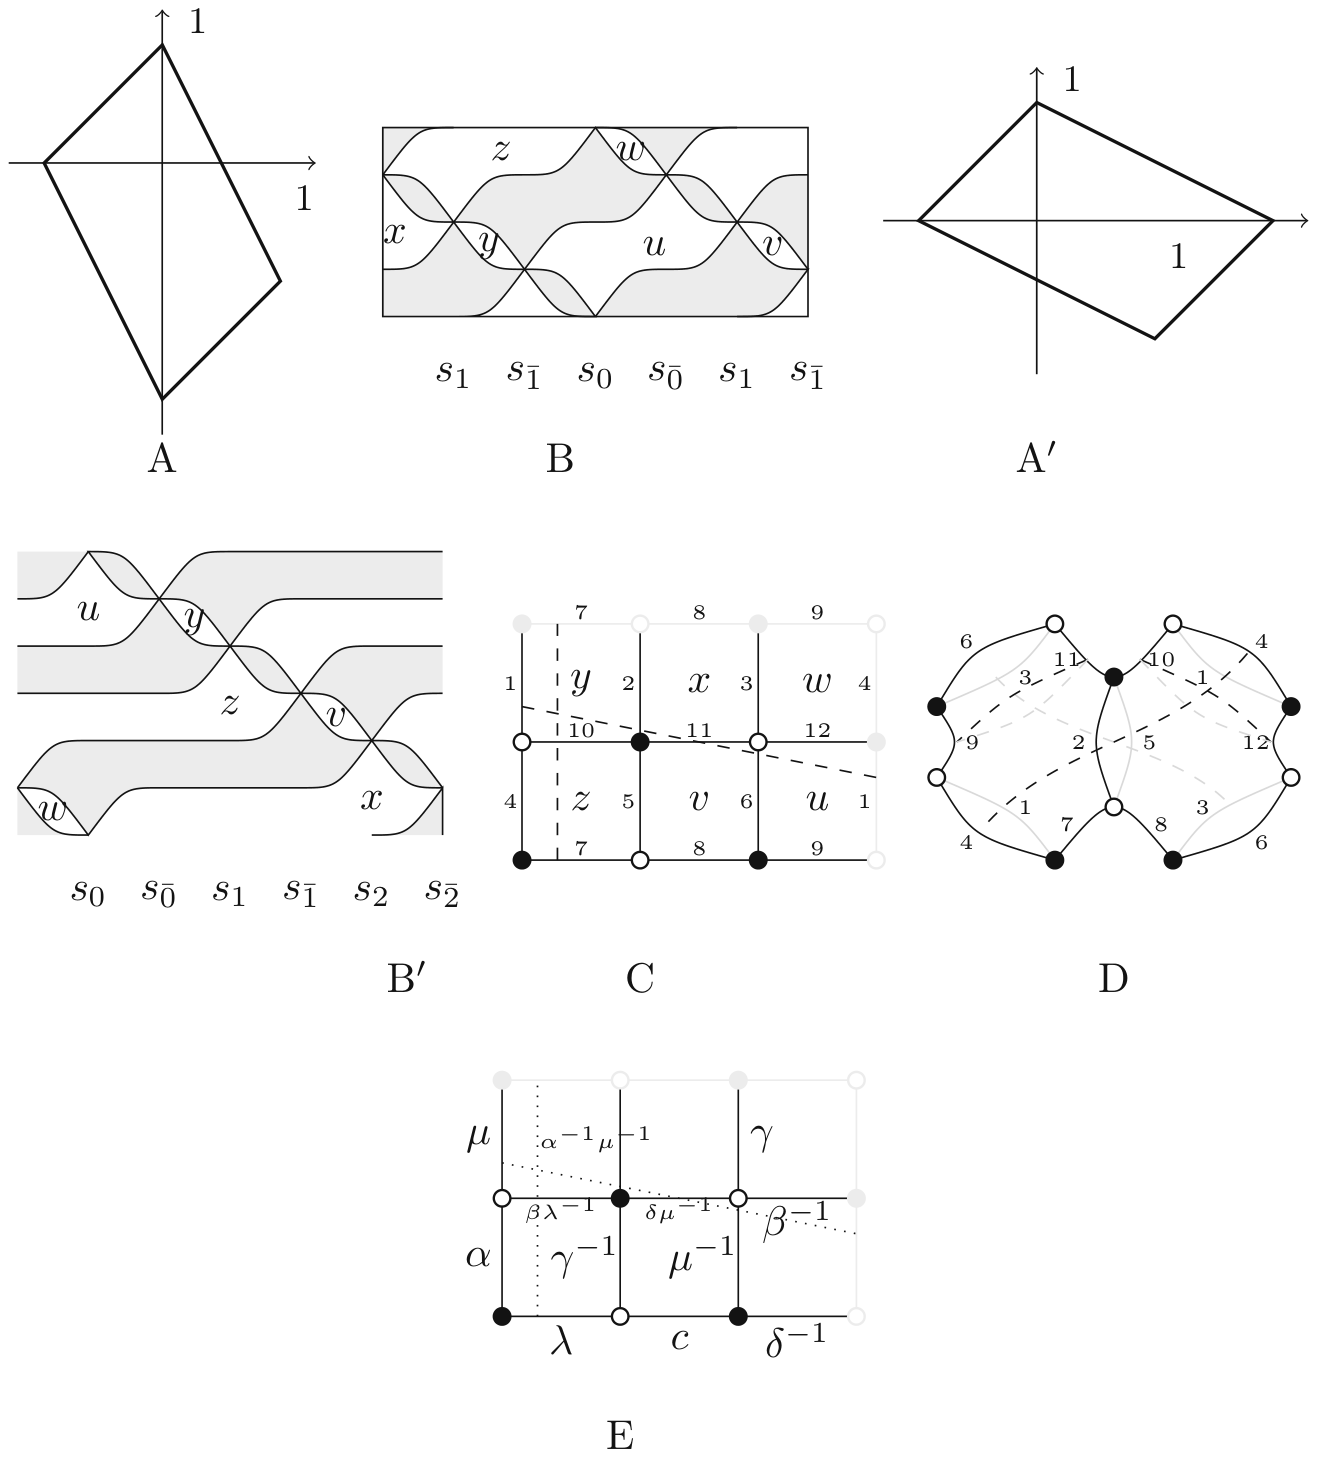
\includegraphics[width=347.7pt]{figs/f1-17.png}
\caption{仿射 $\widehat{PGL}(3)$ 相对论 Toda 链。A：Newton 多边形；B：Thurston 图（左右两边作半转平移后粘合）以及 $\widehat{PGL}(2)$ 的双外尔群中相应的词；$A'$：旋转后的 Newton 多边形；$B'$：旋转后的 Thurston 图以及 $\widehat{PGL}(3)$ 的双外尔群中相应的词；C：环面 $\Sigma$ 上的二部图、两个同调圈与面变量；D：亏格二的对偶曲面 $\tilde\Sigma$ 上的二部图与同调基；E：边变量 $A_e=A_e(\lambda,\mu;\alpha,\beta,\gamma,\delta;c)$。}
\label{fig:1.17}
\end{figure}

考虑顶点为 $(-1,0)$、$(0,1)$、$(2,0)$、$(1,-1)$ 的 Newton 多边形（平行四边形），见图 1.17A。环面 $\Sigma$ 上相应的 Thurston 图见图 1.17B。施加一个格自同构后，同一 Newton 多边形可以表为图 1.17A$'$ 中的平行四边形。对应于图 1.17A$'$ 的 Thurston 图（图 1.17B$'$）与图 1.17B 的 Thurston 图只差一个环面自同构；然而，把图 1.17B 与图 1.17B$'$ 中的环面沿竖直方向剪开后，双外尔群生成元中相应的词并不相同，甚至属于不同的群。前者属于 $\widehat{PSL}(2)$ 的双外尔群，而后者得到的是 $\widehat{PSL}(3)$。这当然是关于 Toda 链的众所周知的事实：Toda 链可以用 $2\times2$ 或 $N\times N$ 的 Lax 矩阵描述，本例中 $N=3$（更多细节与文献见 [21]）；在这里，它来自把环面 $\Sigma$ 沿两种不同方式剪开的可能性。

环面上同调 $H^1(\Sigma)$ 的坐标为 $\lambda$ 与 $\mu$，对应于图 1.17C 中所示的圈。对偶曲面上同调 $H^1(\tilde\Sigma)$ 的生成元 $\alpha$、$\beta$、$\gamma$、$\delta$ 对应于图 1.17D 中所示的圈。

由图 1.17B 或图 1.17B$'$ 中的 Thurston 图得到的面变量之间的 Poisson 括号为：
\[
\begin{gathered}
\{y,z\}=2yz,\qquad \{v,x\}=2vx,\qquad \{w,u\}=2yz,\\
\{z,v\}=zv,\qquad \{z,w\}=zw,\qquad \{x,y\}=xy,\\
\{x,w\}=xw,\qquad \{u,y\}=uy,\qquad \{u,w\}=uw,
\end{gathered}
\]
而其余各对变量都 Poisson 交换。\begin{annote}末式 $\{w,u\}=2yz$ 与同一列表中的 $\{u,w\}=uw$ 不能同时成立（Poisson 括号反对称），且与其余各式“系数为 2 或 1 的单项式”的体例不合，疑为 $\{w,u\}=2wu$（或 $2uw$）之误；译文照排原文。[来源：上下文推断] \end{annote}这个 Poisson 结构可以由对偶于图 1.17C 中二部图的交换图编码，也可以由仿射 $\widehat{PSL}(3)$ 的嘉当矩阵编码。

\begin{figure}[htbp]
\centering
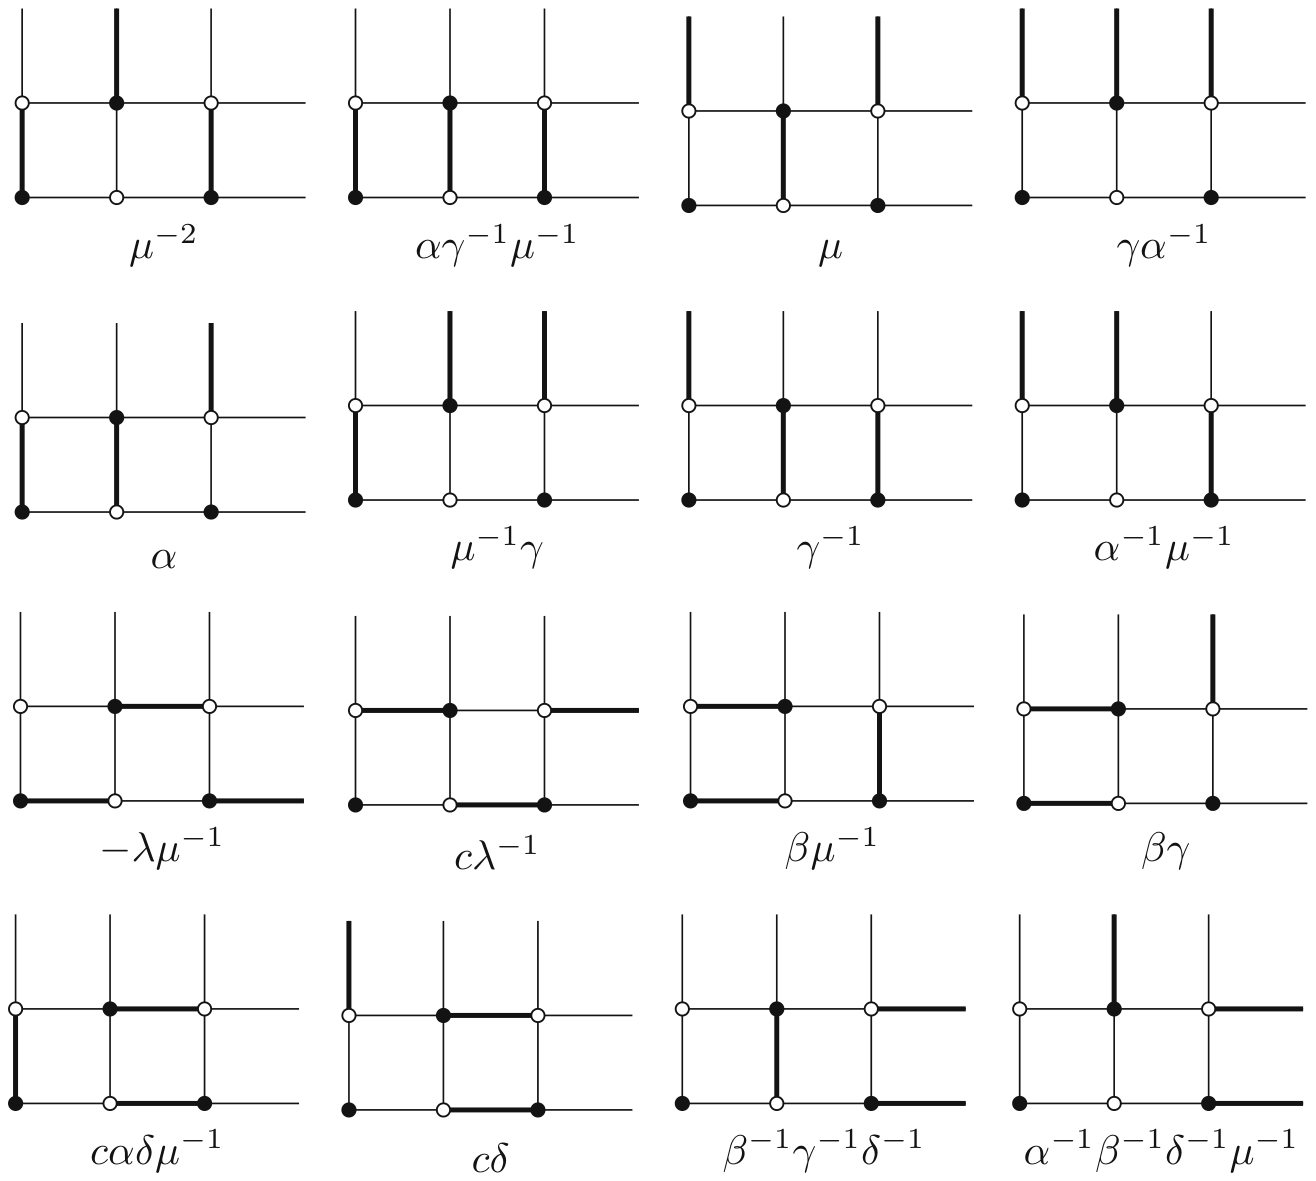
\includegraphics[width=347.4pt]{figs/f1-18.png}
\caption{二聚体构型与配对 $(-1)^{Q(D)}\langle A,D\rangle$。}
\label{fig:1.18}
\end{figure}

共有十六个二聚体构型，见图 1.18，它们求和得到双配分函数：
\begin{equation}
\begin{aligned}
S^d={}&\mu^{-2}+\mu+\mu^{-1}\bigl(\alpha\gamma^{-1}+\gamma+\alpha^{-1}+\beta+c\alpha\delta+\alpha^{-1}\beta^{-1}\delta^{-1}\bigr)\\
&+\bigl(\gamma\alpha^{-1}+\alpha+\gamma^{-1}+\beta\gamma+c\delta+\gamma^{-1}\beta^{-1}\delta^{-1}\bigr)+c\lambda^{-1}-\lambda\mu^{-1}.
\end{aligned}
\tag{1.40}\label{eq:1.40}
\end{equation}

比较图 1.17C 与图 1.17E，可以看出面变量与上同调变量之间的关系为 $x=c^{-1}\alpha^{-1}\gamma\delta^{-1}$，$y=\alpha\beta$，$z=\alpha\beta^{-1}\gamma^{-1}$，$u=\beta\delta$，$v=c\gamma\delta$，$w=(\alpha\beta\gamma\delta)^{-1}$。把这些关系对后一组变量解出，并代入 (1.40)，即得面配分函数
\begin{equation}
\begin{aligned}
S^f={}&\mu^{-2}+\mu+\mu^{-1}c^{1/3}(u^2y^2zv)^{-1/3}\bigl(1+u+uy+uyz+uyzv+c^{-1}yv\bigr)\\
&+c^{1/3}(xyu^2v^2)^{-1/3}\bigl(1+u+uv+uvx+uvxy+c^{-1}uv\bigr)+c\lambda^{-1}-\lambda\mu^{-1}.
\end{aligned}
\tag{1.41}\label{eq:1.41}
\end{equation}

另一方面，同一配分函数在相差一个归一化的意义下由特征多项式给出，而该特征多项式可以从图 1.17B 的词读出。在移位算子取某种方便位置之后计算 $2\times2$ 行列式，得到表达式
\begin{equation}
\begin{aligned}
&\det\bigl(H_1(x)E_1H_1(y)E_{\bar1}H_0(z)E_0(\lambda)H_0(w)E_{\bar0}(\lambda)H_1(u)E_1H_1(v)E_{\bar1}\Lambda-\mu\bigr)\\
&\quad=\mu^2-\lambda\mu x(1+u+uy+uyz+uyzv+uyzvx)\\
&\qquad-\mu(1+u+uv+uvx+uvxy+uvxyz)-\lambda^2\mu x^2yzu-\lambda^{-1}\mu uv-\lambda xuyv,
\end{aligned}
\tag{1.42}\label{eq:1.42}
\end{equation}
它在替换
\[
\lambda\mapsto\mu^{-1}x^{-2/3}y^{-1/3}z^{-1/3}v^{1/3},\qquad
\mu\mapsto\lambda\mu^{-1}x^{2/3}y^{1/3}z^{1/3}uv^{2/3}
\]
下，并在把整个表达式 (1.42) 乘以 $-\lambda^{-1}\mu x^{-4/3}y^{-2/3}z^{-2/3}u^{-2}v^{-4/3}$ 之后，化为 (1.41)。

同一面配分函数也可以从 $3\times3$ 矩阵的特征多项式得到，该矩阵从图 1.17B$'$ 的词读出。计算行列式，并在把所有移位算子推到右边之后，得到
\begin{equation}
\begin{aligned}
&-\det\bigl(H_0(w)E_0(\lambda)H_0(u)E_{\bar0}(\lambda)H_1(y)E_1H_1(z)E_{\bar1}H_2(v)E_2H_2(x)E_{\bar2}-\mu\bigr)\\
&\quad=\mu^3-vwy\mu^2\lambda-(1+u+uv+uvx+uvxy+uvxyz)u^{-1}\mu^2\\
&\qquad+(1+u+uy+uyz+uyzv+uyzvx)vxu^{-1}\mu-vxu^{-1}w^{-1}\mu\lambda^{-1}-v^2x^2yz.
\end{aligned}
\tag{1.43}\label{eq:1.43}
\end{equation}
作替换
\[
\mu\mapsto-\mu x^{2/3}y^{1/3}z^{1/3}v^{2/3},\qquad
\lambda\mapsto\lambda^{-1}x^{2/3}y^{1/3}z^{1/3}v^{2/3},
\]
并把表达式 (1.43) 乘以 $\mu^{-2}x^{-2}y^{-1}z^{-1}v^{-2}$，就回到 (1.41)。

对称群 $\mathcal G'_\Delta=\mathcal G_\Delta$ 的秩为 1、挠为 $\Z/3\Z$。挠生成元 $(0,1,1,0)$ 是置换 $(x,y,z,u,v,w)\mapsto(u,v,x,z,w,y)$。无限阶生成元 $(0,1,0,0)$ 是把 $(x,y,z,u,v,w)$ 映为
\[
\Bigl(y\frac{(1+x)(1+u)}{(1+z^{-1})^2},\ x^{-1},\ v\frac{(1+u)(1+z)}{(1+x^{-1})^2},\ u^{-1},\ w\frac{(1+z)(1+x)}{(1+u^{-1})^2},\ z^{-1}\Bigr)
\]
的变换 $\tau$。

\subsection{任意大小的平行四边形与五角星映射}

最后我们考虑 Newton 多边形为任意大小平行四边形的那一类可积系统。对 $G=\widehat{PSL}(N)$，词
\[
s_0s_{\bar0}s_1s_{\bar1}\cdots s_{l-1}s_{\overline{l-1}}\Lambda^l,
\]
其中下标按模 $N$ 理解，是循环约化的，相应的 Newton 多边形是顶点为 $(0,0)$、$(1,0)$、$(N,l)$、$(N-1,l)$、双面积为 $2l$ 的平行四边形。这样可以得到任一至少有一条本原边的平行四边形。

这里的主要例子将是宽为 3 的平行四边形，即比给出相对论 Toda 格的平行四边形稍宽一点。考虑这样一个例子的主要原因是：这一系统的离散演化由 [26] 发现、由 [22] 研究，是本工作的动因之一。

让我们简要回忆 R. Schwartz 对离散可积系统的构造。考虑射影平面中点序列 $\dots,p_{-1},\allowbreak p_0,p_1,\dots$ 构成的空间。这个空间有一个（双有理的）自同构 $\tau$，由如图 1.19 所示的简单几何构造定义。即：$\tau(p_i)$ 是直线 $(p_{i-1},p_i)$ 与 $(p_{i+1},p_{i+2})$ 的交点。

\begin{figure}[htbp]
\centering
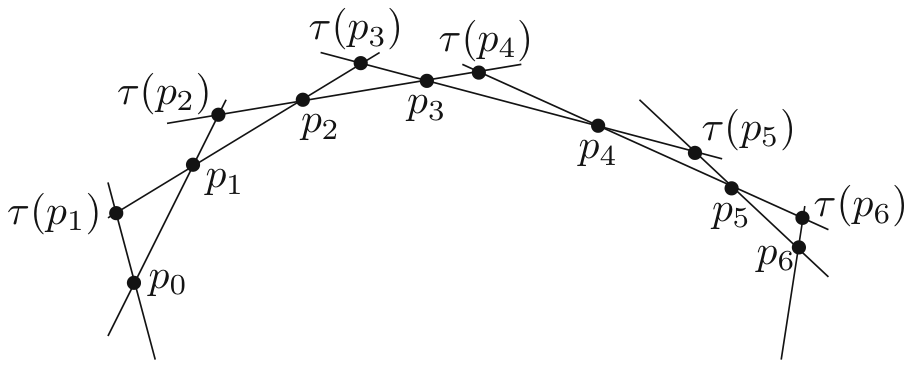
\includegraphics[width=240.8pt]{figs/f1-19.png}
\caption{五角星映射。}
\label{fig:1.19}
\end{figure}

群 $\operatorname{PGL}(3)$ 通过射影变换作用在这个空间上。这样的序列构成的空间包含一个由 $l$-准周期序列的射影类构成的子商，它是有限维的，我们把它记作 $P_l$。所谓 $l$-准周期序列，是指这样的序列 $\dots,p_0,p_1,\dots$：其平移 $\dots,p_l,p_{l+1},\dots$ 与它射影同构。显然，对任意 $l\in\mathbb N$，空间 $P_l$ 的维数为 $2l$。

我们的目标是证明：$P_l$ 典范同构于 $\widehat{PGL}(3)$ 中对应于词 $u=\bigl(\prod_{i=1}^{l}s_is_{\bar i}\bigr)\Lambda^l\in(\tilde W\times\tilde W)^{\sharp}$ 的双 Bruhat 胞腔，其中所有下标都按模 3 理解。此外，我们还将验证：五角星映射 $\tau$ 恰是 §1.7 所述离散流的一个特例。

对 $\RP^2$ 中一般的点序列 $\dots,p_1,p_2,\dots$，可以把它提升为 $\R^3$ 中的一族向量 $\dots,e_1,e_2,\dots$，要求 $e_i+e_{i+1}$ 属于 $e_{i+2}$ 与 $e_{i+3}$ 张成的平面；也就是说，存在系数 $a_i$、$b_i$，使得
\begin{equation}
e_{i+3}=a_i(e_{i+1}+e_i)+b_ie_{i+2}.
\tag{1.44}\label{eq:1.44}
\end{equation}
从基 $e_i,e_{i+1},e_{i+2}$ 到基 $e_{i+1},e_{i+2},e_{i+3}$ 的转移矩阵为
\begin{equation}
M_i=\begin{pmatrix}
0&0&a_i\\
1&0&a_i\\
0&1&b_i
\end{pmatrix}.
\tag{1.45}\label{eq:1.45}
\end{equation}

回忆 R. Schwartz [26] 在射影平面中点序列空间上引入的坐标\footnote{我们的下标约定与 [26] 相差 2。}。对每个 $i$，令 $x_i$ 与 $y_i$ 为共线四点组的交比（cross-ratio）：
\[
\begin{aligned}
x_i&=[p_i,p_{i+1},(p_i,p_{i+1})\cap(p_{i+2},p_{i+3}),(p_i,p_{i+1})\cap(p_{i+3},p_{i+4})],\\
y_i&=[(p_{i+4},p_{i+3})\cap(p_i,p_{i+1}),(p_{i+4},p_{i+3})\cap(p_{i+1},p_{i+2}),p_{i+3},p_{i+4}].
\end{aligned}
\]
这里 $(p_i,p_j)$ 表示过 $p_i$ 与 $p_j$ 的直线；交比取为
\[
[a,b,c,d]=\frac{(a-b)(c-d)}{(a-c)(b-d)}.
\]

Schwartz 坐标 $x_i$ 与 $y_i$ 可以（见附录 1.14 中的 (1.58)）按
\begin{equation}
x_i=\frac{b_i}{a_i},\qquad y_i=-\frac{a_{i+1}}{b_ib_{i+1}}
\tag{1.46}\label{eq:1.46}
\end{equation}
计算。反之，
\begin{equation}
a_i=-(x_ix_{i+1}y_i)^{-1},\qquad b_i=-(x_{i+1}y_i)^{-1},
\tag{1.47}\label{eq:1.47}
\end{equation}
于是表达式 (1.45) 在 Schwartz 坐标下（差一个标量倍数）为
\begin{equation}
M_i=\begin{pmatrix}
0&0&x_i^{-1}\\
-y_ix_{i+1}&0&x_i^{-1}\\
0&-y_ix_{i+1}&1
\end{pmatrix}.
\tag{1.48}\label{eq:1.48}
\end{equation}

因此，从 $e_k,e_{k+1},e_{k+2}$ 到 $e_m,e_{m+1},e_{m+2}$ 的转移矩阵由矩阵 (1.48) 的乘积
\begin{equation}
M_{k\to m}=M_kM_{k+1}\cdots M_{m-1}
\tag{1.49}\label{eq:1.49}
\end{equation}
给出。

我们的关键观察是：转移矩阵 $M_{k\to m}$ 可以写成群 $\widehat{PSL}^{\sharp}(3,\R)$ 的生成元的一个简单表达式。即，考虑乘积
\begin{equation}
\begin{aligned}
\hat M(u,v,\lambda)&=H_0(u)E_0\Lambda E_{\bar0}H_2(v)\\
&=T_u\begin{pmatrix}1&0&0\\0&1&0\\ \lambda&0&1\end{pmatrix}
\begin{pmatrix}0&0&\lambda^{-1}\\1&0&0\\0&1&0\end{pmatrix}
\begin{pmatrix}1&0&\lambda^{-1}\\0&1&0\\0&0&1\end{pmatrix}
\begin{pmatrix}v&0&0\\0&v&0\\0&0&1\end{pmatrix}T_v\\
&=\begin{pmatrix}0&0&\lambda^{-1}u^{-1}\\ v&0&\lambda^{-1}u^{-1}\\0&v&1\end{pmatrix}T_{uv}=M(u,v,\lambda)T_{uv}.
\end{aligned}
\tag{1.50}\label{eq:1.50}
\end{equation}

这个表达式的矩阵部分与矩阵 (1.48) 直接相关：
\[
M_i=M(a_i/b_i,1/b_i,1)=M(x_i,y_ix_{i+1},1),
\]
并且它具有显然的性质 $T_wM(u,v,\lambda)=M(uw,v,\lambda)T_w$。因此，乘积
\[
\hat M(u_k,v_k,\lambda)\cdots\hat M(u_{m-1},v_{m-1},\lambda)
\]
可以通过把所有移位算子移到右边而化为
\[
\begin{aligned}
&\hat M(u_k,v_k,\lambda)\cdots\hat M(u_{m-1},v_{m-1},\lambda)\\
&\quad=M(u_k,v_k,\lambda)M(u_{k+1}v_ku_k,v_{k+1},\lambda)\cdots\\
&\qquad\cdot M(u_{m-1}v_{m-2}u_{m-2}\cdots v_ku_k,v_{m-1},\lambda)\,T_{u_kv_k\cdots u_{m-1}v_{m-1}}.
\end{aligned}
\]
把这个表达式与代入 (1.48) 后的乘积 (1.49)
\[
M_{k\to m}=M(x_k,-y_kx_{k+1},1)\cdots M(x_m,-y_mx_{m+1},1)
\]
相比较，可以看出，在等同
\begin{equation}
u_i=-(x_{i-1}y_{i-1})^{-1},\qquad v_i=-y_ix_{i+1}
\tag{1.51}\label{eq:1.51}
\end{equation}
之下二者一致。

变量 $u_i$ 与 $v_i$ 是由 M. Glick 在 [10] 中引入的点序列空间上的坐标，他在其中证明：五角星映射在这些坐标下是一串变异。

另一方面，乘积 $\hat M(u_k,v_k)\cdots\hat M(u_{m-1},v_{m-1})$ 可以通过把所有自同构 $\Lambda$ 移到右边而化为
\begin{equation}
\begin{aligned}
&\hat M(u_k,v_k)\cdots\hat M(u_{m-1},v_{m-1})\\
&\quad=H_0(u_k)E_0\Lambda E_{\bar0}H^{-1}(v_k)\cdots H_0(u_{m-1})E_0\Lambda E_{\bar0}H^{-1}(v_{m-1})\\
&\quad=H_0(u_k)E_0E_{\bar1}H_0(v_k)\cdots H_{m-k-1}(u_j)E_{m-k-1}E_{m-k}H_{m-k-1}(v_{m-1})\Lambda^{m-k}.
\end{aligned}
\tag{1.52}\label{eq:1.52}
\end{equation}
\begin{annote}第二行末 $H_{m-k-1}(u_j)$ 中的下标 $u_j$ 在原文中即如此，但从乘积结构看它应与本行的其余项一致而取 $u_{m-k-1}$；译文照排原文。[来源：上下文推断]
\end{annote}

因此，这个表达式就是映射 (1.21) 的标准表达式，它对应于词
\[
u=s_0s_{\bar1}s_1s_{\bar2}s_2\cdots s_{m-k-1}s_{m-k}\Lambda^{m-k},
\]
该词显然是循环约化的。按照附录 1.11 的标准规则，Poisson 括号与 [10] 中的相同：
\begin{equation}
\begin{aligned}
\{u_j,v_i\}&=u_jv_i &\text{若 } j=i+2 \text{ 或 } j=i-1,\\
\{u_j,v_i\}&=-u_jv_i &\text{若 } j=i \text{ 或 } j=i+1,
\end{aligned}
\tag{1.53}\label{eq:1.53}
\end{equation}
而其余所有括号为零。(1.52) 的特征多项式给出谱曲线，其 Newton 多边形是宽为 3（$3\times3$ 矩阵）、长度任意的平行四边形，见 [21]。

\paragraph{五角星映射}
现在考虑五角星映射 $\tau$。按照映射的定义以及我们的向量序列 $\{e_i\}$ 的归一化 (1.44)，演化后的基 $\{\tilde e_i=\tau(e_i)\}$ 应由简单公式 $\tilde e_i=\alpha_i(e_{i+1}+e_i)$ 给出，其中 $\alpha_i$ 是非零常数。另一方面，序列的新坐标 $\tilde a_i$ 与 $\tilde b_i$ 由关系 $\tilde e_{i+3}=\tilde a_i(\tilde e_{i+1}+\tilde e_i)+\tilde b_i\tilde e_{i+2}$ 定义。把这些关系合在一起，就得到五角星映射的显式表达式（见附录 1.14）：
\begin{equation}
\alpha_i=\frac{a_i}{b_{i+1}},\qquad
a_i\mapsto\tilde a_i=a_{i+3}\frac{b_{i+1}+1}{b_{i+3}+1},\qquad
b_i\mapsto\tilde b_i=b_i\frac{(b_{i+1}+1)(b_{i+2}+1)a_{i+3}}{(b_i+1)(b_{i+3}+1)a_{i+2}}.
\tag{1.54}\label{eq:1.54}
\end{equation}
利用 (1.46) 与 (1.47)，在 Schwartz 坐标下得到
\begin{equation}
x_i\mapsto x_{i+2}\frac{1-x_{i+3}y_{i+2}}{1-x_{i+1}y_i},\qquad
y_i\mapsto y_{i+1}\frac{1-x_{i+1}y_i}{1-x_{i+3}y_{i+2}},
\tag{1.55}\label{eq:1.55}
\end{equation}
它与 [26, p.~523] 或 [22, 公式 (2.5)] 相差一个指标移位后一致。

用簇坐标 $u_i$ 与 $v_i$ 表出这一演化，得到
\begin{equation}
u_i\mapsto v_{i-1}^{-1},\qquad
v_i\mapsto u_{i+2}(1+v_i)(1+v_{i+3})(1+v_{i+1}^{-1})^{-1}(1+v_{i+2}^{-1})^{-1}.
\tag{1.56}\label{eq:1.56}
\end{equation}
这个变换是这样一个复合：先对所有变量 $v_i$ 作簇变异
\[
v_i\mapsto v_i^{-1},\qquad
u_i\mapsto u_i(1+v_{i-2})(1+v_{i+1})(1+v_{i-1}^{-1})^{-1}(1+v_i^{-1})^{-1},
\]
再作重编号
\[
v_i\mapsto u_{i+2},\qquad u_i\mapsto v_{i-1}.
\]

\paragraph{其他维数}
注意，若把 $\widehat{PGL}(3)$ 换成 $\widehat{PGL}(N)$（$N\geqslant2$ 任意），该构造仍然成立。对一般的 $N>2$，算子 (1.50) 变为
\[
\hat M=T_u\begin{pmatrix}
0&0&\cdots&0&\lambda^{-1}u\\
v&0&\cdots&0&\lambda^{-1}u\\
0&v&\cdots&0&0\\
\vdots& &\ddots& &\vdots\\
0&0&\cdots&v&1
\end{pmatrix}.
\]
Poisson 括号与 (1.53) 完全类似：
\[
\{u_j,v_i\}=u_jv_i\quad\text{若 } j=i+N-1 \text{ 或 } j=i-1,\qquad
\{u_j,v_i\}=-u_jv_i\quad\text{若 } j=i \text{ 或 } j=i+N-2,
\]
其余为零。对 $N=2$，算子 $\hat M$ 变为
\[
\hat M=T_u\begin{pmatrix}1&0\\ \lambda&1\end{pmatrix}
\begin{pmatrix}0&\lambda^{-1}\\1&0\end{pmatrix}
\begin{pmatrix}1&\lambda^{-1}\\0&1\end{pmatrix}
\begin{pmatrix}v&0\\0&1\end{pmatrix}T_v
=\begin{pmatrix}0&\lambda^{-1}u^{-1}\\ v&\lambda^{-1}u^{-1}+1\end{pmatrix}T_{uv},
\]
而 Poisson 括号变为
\[
\{u_j,v_i\}=u_jv_i\quad(j=i+1 \text{ 或 } i-1),\qquad
\{u_j,v_i\}=-2u_jv_i\quad(j=i),
\]
这已在 §1.8.4 中用到（例如可与 (1.42) 对照）。
